
We consider a (matching) market of $k$ sellers and $k$ buyers, where $k$ is an integer, $k>0$. 
Each seller sells an item and the prices of the items are initially all zero. Buyer $i$ has valuation $k-i+1$ for the first item and valuation $0$ for every other item, as shown in the following diagram.

\vspace*{0.5cm}
\begin{tabular}{c r c c c}
    Buyers & \multicolumn{4}{c}{Valuations (for items $1$ to $k$)} \\
    \hline
    $x_1$ & $k,$ & $0,$ & $\ldots,$ & $0$ \\
    $x_2$ & $k-1,$ & $0,$ & $\ldots,$ & $0$ \\
    $\vdots$ & & & $\vdots$ \\
    $x_k$ & $1,$ & $0,$ & $\ldots,$ & $0$ \\
\end{tabular}

\noindent The sellers find the market-clearing prices using the procedure discussed in the lectures.
\begin{enumerate}
    \item[(a)] What are the prices of the sellers' items ($1^{st}$ item, $2^{nd}$ item, \ldots, $k^{th}$ item) when the market clears? Which buyer gets the $1^{st}$ item and at what price?  \hfill{\bf [3 marks]}\smallskip

    The $1^{st}$ item is sold at a price of $k - 1$.
    The $2^{nd}$ to $k^{th}$ items are sold at a price of $0$.

    Buyer $x_1$ gets the $1^{st}$ item at a price of $k - 1$.

    \item[(b)] Justify your answers to (a).  \hfill{\bf [6 marks]}\smallskip

    Let Algorithm 1 be the procedure for finding market-clearing prices as shown in the lectures and $x_{j,i}$ be the valuation of item $i$ by buyer $j$.

    \begin{theorem}
        The matching market in this case results in the market-clearing prices $(k - 1, 0, \dots, 0)$ for items $1, 2, ..., k$.
    \end{theorem}

    \begin{proof}
        Using induction.

        \underline{Base case ($k = 1$)}:
    
        Applying Algorithm 1, the $1^{st}$ seller's price $p_1$ is initially $0$.
        This trivially produces the following preferred-seller graph since buyer $x_1$ values the item at $1$, giving them a positive payoff of $x_{1,1} - p_1 = 1 - 0 = 1$.

        \hfil
        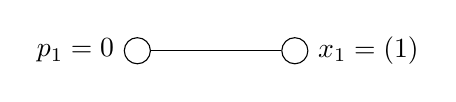
\begin{tikzpicture}[main/.style={circle,draw}]
            \node[main, label={left:$p_1 = 0$}] at (0, 2) (p1) {};

            \node[main, label={right:$x_1 = (1)$}] at (2, 2) (x1) {};

            \draw(p1) -- (x1);
        \end{tikzpicture}
        \hfil

        This is clearly a perfect bipartite matching, hence, for $k = 1$, the theorem holds.

        Next, consider $k = n$ for a positive integer $n$.

        In this case, trivially, any buyer 

        \begin{lemma}
            Any complete bi-partite graph $K_{n, n}, n > 0$ has a perfect matching.
        \end{lemma}
        \begin{proof}
            Trivial, connect left node $i$ to right node $i$ for all $1 \leq i \leq n$.
        \end{proof}

        \hfil
        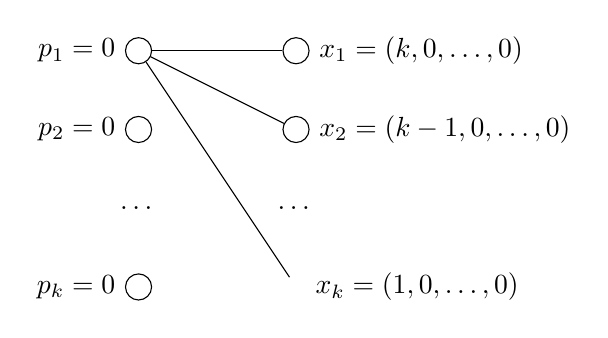
\begin{tikzpicture}[main/.style={circle,draw}]
            \node[main, label={left:$p_1 = 0$}] at (0, 2) (p1) {};
            \node[main, label={left:$p_2 = 0$}] (p2) [below of=p1] {};

            \node (pDots) [below of=p2] {\dots};

            \node[main, label={left:$p_k = 0$}] (pk) [below of=pDots] {};

            \node[main, label={right:$x_1 = (k, 0, \dots, 0)$}] at (2, 2) (x1) {};
            \node[main, label={right:$x_2 = (k - 1, 0, \dots, 0)$}] (x2) [below of=x1] {};

            \node (xDots) [below of=x2] {\dots};

            \node[label={right:$x_k = (1, 0, \dots, 0)$}] (xk) [below of=xDots] {};

            \draw(p1) -- (x1);
            \draw(p1) -- (x2);
            \draw(p1) -- (xk);
        \end{tikzpicture}
        \hfil

        Trivially, a single edge from item 1 to 
        
        \begin{corollary}
            Removing the vertices for seller $1$ and buyer $x_1$ from the preferred-seller graph yields the complete bipartite graph $K_{k - 1,k - 1}$
        \end{corollary}
    \end{proof}

    \item[(c)] Which kind of auction does the construction of market-clearing prices procedure implement in this case?  \hfill{\bf [3 marks]}\smallskip

    As the winner of item $1$ is the buyer ($x_1$ in this case) who values it the highest.
    They pay the valuation of item $1$ by the second highest buyer ($k - 1$ in this case). 
    Thus, the construction of market-clearing prices implements a second-price (Vickrey) auction for item 1 in this case.

\end{enumerate}
